\documentclass[11pt]{scrartcl}
\usepackage[sexy]{{style_files/evan}}

\usepackage{{style_files/NMC}}
\usepackage{standalone}
\usepackage{import}

\begin{document}
\title{NMC Problem Set \#19} % add # of pset
\date{Dec. 25, 2022} % add date
\maketitle

\section*{Welcome!}

This is a selection of interesting problems derived from curious thoughts, curated so you can nibble on them throughout the week! The point of this document is to introduce you to fun puzzles that require thinking. We recommend you try the ones that you find interesting! Feel free to work on them with others (even us teachers!). Harder problems are marked with chilies (\fullchili), in case you want to challenge yourself.
\newline\newline
Have fun! \textit{Note: New variants on these problems may be released throughout the week. Remember to check back once in a while!}
    
\section{Algebra}
\begin{enumerate}[label=\textbf{A\arabic*}.]
    \item \textbf{Detour (Calculus)} \newline
    Suppose we have a real polynomial, $P(x)$, and let $f : \RR \to \RR$ be a function such that $f(f(x)) = P(x)$.
    
    \begin{enumerate}
        \item Suppose we have $P(x) = 2x^3 - 2x^2 + 2x - 1$. Prove that $f$ is not differentiable.

        \item Suppose $f(f(x)) = x$ has the unique solution $a$. Prove that $f(x) = x$ also has the unique solution $a$, then conclude that if $P'(a)$ is negative, $f$ is not differentiable. \footnote{note that this is a sufficient but definitely not a necessary condition by any means}

        \item (\fullchili \hspace{1pt} $\times$ Open) For which choices of polynomial $P(x)$ will we have a non-differentiable $f$?
    \end{enumerate}

    \item \textbf{French Functions} \newline
    Call a continuous function \textit{French} if $f(f(x)) = 2f(x) - x$ for all $x$. Determine all such \textit{French} functions.
    
\end{enumerate}

\newpage
\section{Combinatorics}
\begin{enumerate}[label=\textbf{C\arabic*}.]
    \item \textbf{Snake Game} \newline
    Suppose we are playing the snake on an $m \times n$ board. Here's a \href{https://en.wikipedia.org/wiki/Snake_(video_game_genre)}{link} to how said game works!

    \begin{enumerate}
        \item Define a win position to be a board where the snake covers all $mn$ squares. How many possible different win positions are there for $m, n = 3, 4, 5$?
    
        \item (\fullchili \hspace{1pt} $\times$ Open) Determine the exact number of win positions for any choice of naturals $m, n$. This is the same as asking for the number of Hamiltonian paths on a rectangular lattice of the same dimensions.
    \end{enumerate}

    \item \textbf{Selection} \newline
    A group of friends contains $n$ people. If the number of ways of selecting $6$ friends from the group is the same as the number of ways to select $9$, find the number of ways to select $4$ friends.
    
\end{enumerate}

\newpage
\section{Geometry}
\begin{enumerate}[label=\textbf{G\arabic*}.]
    \item (\fullchili) \textbf{Hypersphere} \newline
    Suppose we have a $d$-dimensional unit hypersphere. Provide an intuitive argument on why, as $d \to \infty$, the volume of said hypersphere approaches 0.

    \item \textbf{Staring at Polyhedra} \newline
    Prove that for any polyhedron $P$ with $n$ faces, there is always at least one way to "look" at it so that you can see $n/2$ faces. Also prove the maximum possible number of faces you can see at once is $n-1$. Here's an example below:

    \begin{figure}[h]
        \centering
        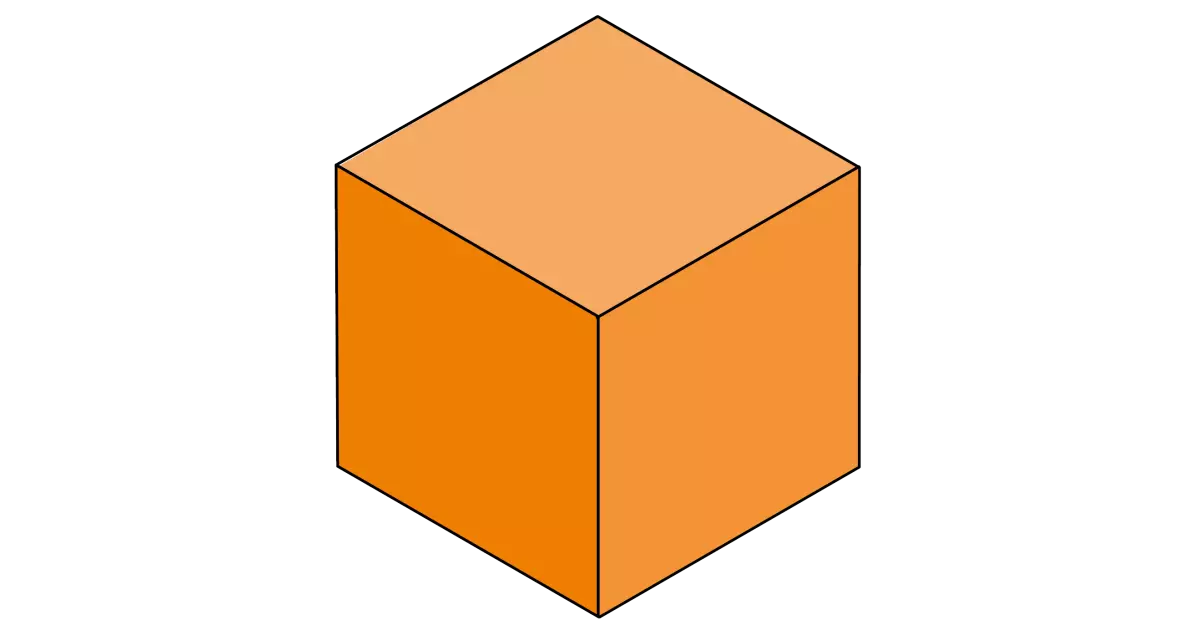
\includegraphics[width = 8.9cm]{Diagrams/Cube.png} % 15cm = aligned?
        \caption{Here, we can see $3$ visible sides of the cube.}
        \label{fig:Cube}
    \end{figure}    
\end{enumerate}

\newpage
\section{Number Theory}
\begin{enumerate}[label=\textbf{N\arabic*}.]
    \item \textbf{Nice Dates} \newline
    It's nearly 2023! We call a day \textit{nice} if, when the date is written out in the form $YYYY/DD/MM$, the number
    \[ \frac{YYYY}{DD/MM} \]
    is an integer. How many nice days does $2023$ have and has there been a nicer year in the past century? The "niceness" of a year is defined by how many nice days it has.
    \footnote{DMO Daily}

    \item \textbf{How Santa Determines if a Kid is Naughty or Nice} \newline
    Suppose we have a sequence $(a_n)$, with $a_1 = 1$. Let $a_n$ be defined as the least positive integer not equal to $a_i$ or $a_i + i$ for all $i < n$. 

    \begin{enumerate}
        \item Show that $a_n = \floor{n\varphi}$.

        \item (\fullchili) Should Santa only deliver gifts to children whose address contains some number from $(a_n)$? Provide a $3000$ word philosophical essay detailing the ethics of selective gift-giving and the ramifications of civil lawsuits on jealousy and selfishness. \footnote{what did i do here idk}
    \end{enumerate}
    
\end{enumerate}

\end{document}
